\chapter{艇员管理系统}
A crew management system can store the training record and provide a great feed
back for the training crew. Our crew is training on a daily basis, one finds
that by comparing and contrast, would make a positive and huge impact on the
confidence and momentum of he training individuals as well as crew members.
In the old school ways, our crew members have to use pen and paper to write down
their training results, and later need to be typed into computers. Therefore
developing a crew management system would greatly enhance the efficiency in
terms of designing training plans and logging training results
.
艇员管理系统是一个能够发布训练计划,统计训练记录的系统。并能通过统计得到的训练记
录进行反馈,为队员提供参考。一个体育团队通过收集每天的训练情况来定期给队员提供积
极科学的反馈,并以此能够修正训练计划,从而使训练更加高效有序。可是现实团队里面在
即时通讯软件(wechat)里面发布和收集训练记录,或者说用纸来记录数据。这样的做法费
时费力而且数据也不完整,即使通信软件里面有相当强大的搜索功能。但是如果每次进行数
据收集都是对聊天记录进行搜索的话,数据难免丢失(数据格式不一致等原因)因此开发一
个数据库应用来进行队内事务管理是相当有必要的。

\newpage

\section{开发环境与开发工具}

\section{系统需求分析}% need further investigation, query somebody maybe
% \begin{enumerate}
% \item
%   {system user management
%     \begin{enumerate}
%     \item{user adding\\
%         include 3 kinds of member type: Crew Coach, Crew Leader, Crew member\\
        
%         Crew Coach can announce the plans for this year: have access to
%         modifying the calender: dates for group extra training program, dates for out
%         field races, etc..\\
        
%         Crew Leader can design and publish training plans(in the form of
%         notice-board) and specify the training program for the day. Have access
%         to team budgets, logging of team budgets.\\
        
%         Crew members can update their status on the training program of the day.
%         How many push-ups and squats(training programs of the day), how much time
%         for the 10 laps running, etc..\\

%         Crew member information: Entrance date, height, weight, age.
        
%         To be continued...
%         }
%       \item{user deletion\\
%           the deletion of the mentioned crew member types. Cascade deletion(deleting
%           team members would also delete their training records)
%         }
%       \item{password modification
%           add password, update password. Involves registration.\\
%         }
%     \end{enumerate}
%   }

% \item{training plans management\\
%     training plans CRUD(Create, Read, Update, Delete):
%   }

% \item {
%     training log management\\
%     training log CRUD
%   }

% \item {
%     Crew members information management\\
%     crew members information CRUD
%   }

% \item {
    
%   }
  
% \end{enumerate}

\begin{enumerate}
\item
  {系统的用户管理\\
    包括用户的添加、删除、修改信息、修改密码等。}

\item{艇员信息管理\\
    艇员信息的添加、删除、修改、查询。
  }

\item{训练计划管理\\
    训练计划的添加,修改,删除,查询。
  }

\item {训练记录管理\\
    训练记录的添加,修改,删除,查询。
  }

\item {船艇信息\\
    艇的信息添加,修改,删除,查询。
  }

\item {开支信息\\
    开支记录的添加,修改,删除,查询。
  }

\end{enumerate}





%making the blow text smaller perhaps?

\section{功能需求分析}
艇员管理系统按照上面所述,管理功能主要在艇员信息、训练计划和训练记录的管理上面。
下面还有一些主要的功能说明
\begin{enumerate}
\item{其中用户分为两个级别。普通用户级别和特权用户级别。特权用户级别的操作是普通用户级别的超集。}

\item{其中添加、删除操作输入特权用户级别,AKA只有特权用户能够添加新的成员。而每个用户需要自己的艇员信息被录入才能注册新的用户。每个用户能够对自己的信息进行查询,对部分信息能够进行修改。}

\item{其中添加,修改,删除属于特权用户级别。}

\item{每个用户只能对自己的训练记录进行(CUD--Create, Update, Delete)。每个用户可以查询其他用户的训练记录。}

\item{普通用户只能部分修改,能够查询。}
\end{enumerate}


\section{系统设计}

% \usetikzlibrary{shapes.geometric, arrows, decorations.markings}
\usetikzlibrary{arrows,decorations.pathmorphing,backgrounds,positioning,fit,petri,
shapes.geometric, decorations.markings}

\tikzstyle{vecArrow} = [thick, decoration={markings,mark=at position
   1 with {\arrow[semithick]{open triangle 60}}},
   double distance=1.4pt, shorten >= 5.5pt,
   preaction = {decorate},
   postaction = {draw,line width=1.4pt, white,shorten >= 4.5pt}]

\tikzstyle{entity} = [rectangle, minimum width=3cm, minimum height=1cm,
                      text width=3cm,
                      fill=white,
                      draw=black,
                      text centered,
                      top color=gray,
                      opacity=0.5,
                      bottom color=white]
                      
\tikzstyle{relationship} = [diamond, minimum width=3cm, minimum height=1cm,
                      text width=3cm,
                      fill=white,
                      draw=black]

\tikzstyle{attribute} = [rectangle, minimum width=3cm, minimum height=1cm,
                      text width=3cm,
                      fill=white,
                      draw=black]
                      

% \tikzstyle{attribute} = [top color=white, bottom color=yellow!20, 
%                                draw=yellow, node distance=1cm]
\tikzstyle{isa} = [top color=white, bottom color=green!20, 
                         draw=green!50!black!100]


\centering
\scalebox{.5}{
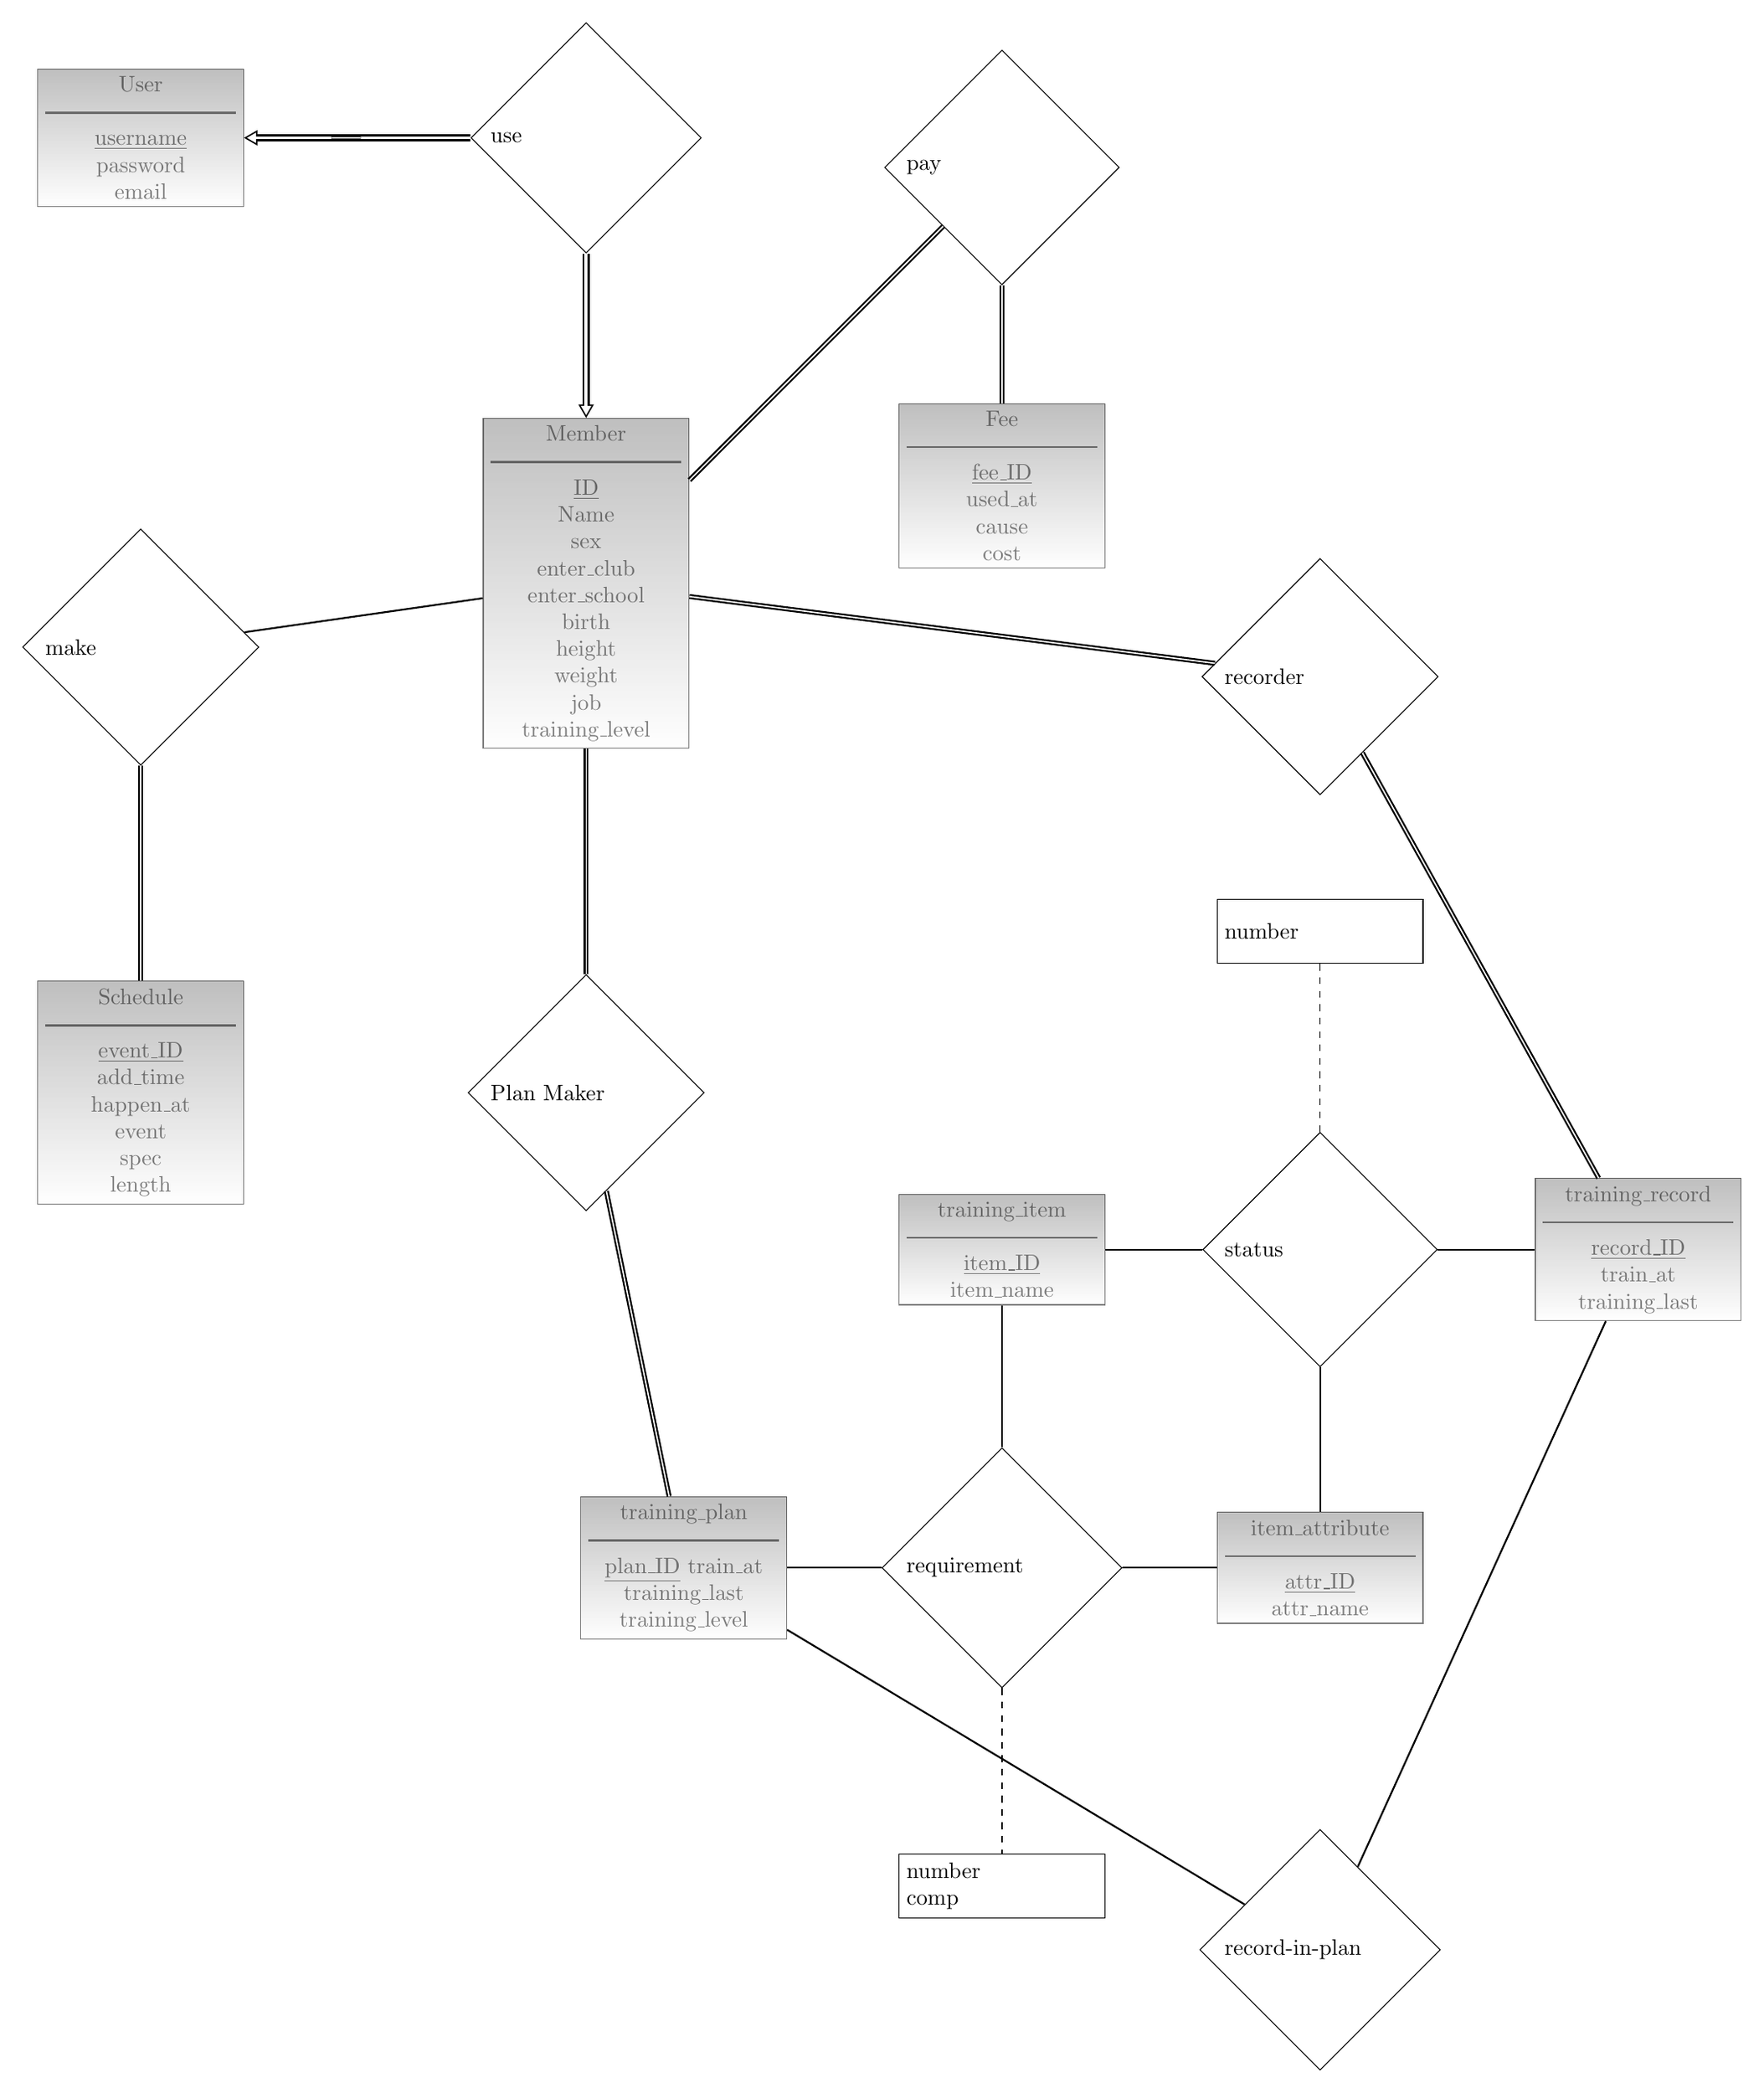
\begin{tikzpicture}[node distance=5cm]

  \node (user) [entity, xshift=-3cm] {
    User\\
    \noindent\rule[0.5ex]{3cm}{1pt}
    
    \underline{username}\\
    password\\
    email\\
  };

  \node (use) [relationship, right of=user, xshift=2cm] {
    use
  };

  \node (member) [entity, below of=use, yshift=-2cm] {
    Member \\
    \noindent\rule[0.5ex]{3cm}{1pt}

    \underline{ID}\\
    Name\\
    sex\\
    enter\_club\\
    enter\_school\\
    birth\\
    height\\
    weight\\
    job\\
    training\_level\\
  };

  \draw[vecArrow] (use) to (user);
  \draw[vecArrow] (use) to (member);

  %   \draw[thick, double](0,0)--(3ex,0) (use) to (user);
  % \draw[thick, double](0,0)--(3ex,0) (use) to (member);


  \node (schedule) [entity, below of=user, yshift=-10cm] {
    Schedule\\
    \noindent\rule[0.5ex]{3cm}{1pt}

    \underline{event\_ID}\\
    add\_time\\
    happen\_at\\
    event\\
    spec\\
    length\\
  };

  \node (make) [relationship, below of=user, yshift=-3cm] {
    make
  };

  \draw[thick, double](0,0)--(3ex,0) (make) to (schedule);
  \draw[thick] (make) to (member);

  \node(pay) [relationship, above right of=member, xshift=3cm, yshift=3cm] {
    pay
  };

  \node (fee) [entity, below of=pay] {
    Fee\\
    \noindent\rule[0.5ex]{3cm}{1pt}

    \underline{fee\_ID}\\
    used\_at\\
    cause\\
    cost\\
  };


  \draw[thick, double](0,0)--(3ex,0) (pay) to (fee);
  \draw[thick, double](0,0)--(3ex,0) (pay) to (member);

  \node (item) [entity, below of=fee, yshift=-7cm] {
    training\_item\\
    \noindent\rule[0.5ex]{3cm}{1pt}
    
    \underline{item\_ID}\\
    item\_name\\
  };

  \node(requirement) [relationship, below of=item] {
    requirement
  };

  \node(status) [relationship, right of=item] {
    status
  };

  \node(req-attr) [attribute, below of=requirement] {
    number\\
    comp
  };

  \node(sta-attr) [attribute, above of=status] {
    number\\
  };

  \node (record) [entity, right of=status] {
    training\_record\\
    \noindent\rule[0.5ex]{3cm}{1pt}

    \underline{record\_ID}\\
    train\_at\\
    training\_last\\
  };

  \node (plan) [entity, left of=requirement] {
    training\_plan\\
    \noindent\rule[0.5ex]{3cm}{1pt}
    
    \underline{plan\_ID}
    train\_at\\
    training\_last\\
    training\_level\\ % take note here, need changes
  };

  \node (attribute) [entity, right of=requirement] {
    item\_attribute\\
    \noindent\rule[0.5ex]{3cm}{1pt}

    \underline{attr\_ID}\\
    attr\_name\\
  };

  \draw[thick] (requirement) to (plan);
  \draw[thick] (requirement) to (item);
  \draw[thick] (requirement) to (attribute);

  \draw[thick] (status) to (item);
  \draw[thick] (status) to (attribute);
  \draw[thick] (status) to (record);
  
  \draw[dashed] (requirement) to (req-attr);
  \draw[dashed] (status) to (sta-attr);

  \node(plan-maker) [relationship, below of=member, yshift=-3cm] {
    Plan Maker
  };

  \node(recorder) [relationship, right of=fee, yshift=-3cm] {
    recorder
  };

  \draw[thick, double](0,0)--(3ex,0) (plan-maker) to (plan);
  \draw[thick, double](0,0)--(3ex,0) (plan-maker) to (member);

  \draw[thick, double](0,0)--(3ex,0) (recorder) to (record);
  \draw[thick, double](0,0)--(3ex,0) (recorder) to (member);
  
  \node(record-in-plan) [relationship, below of=attribute, yshift=-1cm] {
    record-in-plan
  };

  \draw[thick] (record-in-plan) to (record);
  \draw[thick] (record-in-plan) to (plan);

  % \node(ship) [entity] {
  %   ship\\
  %   \noindent\rule[0.5ex]{3cm}{1pt}
    
  %   \underline{name}\\
  %   condition\\
  % };

  % \node(ship type) [entity, right of=ship] {
  %   ship\_type\\
  %   \noindent\rule[0.5ex]{3cm}{1pt}

  %   type\_ID\\
  %   ship\_type\_name\\
  % };
      
\end{tikzpicture}
}
\newpage
\tikzstyle{block}=[rectangle,draw=black,fill=white,text centered, anchor=north,
minimum width=3cm]

\tikzstyle{myarray}=[->,>=open triangle 90, thick]

\begin{center}
  \scalebox{.75} {
    \begin{tikzpicture}[node distance=5cm]

      \node(main) [block, xshift=-5cm]{艇员管理系统};

      \node(user) [block, above right of=main, xshift=2cm]{系统管理};
      % ========================================
      \node(login) [block, above right of=user, xshift=2cm, yshift=-2cm]{用户登录};
      \node(logout) [block, below of=login, yshift=4cm]{用户登出};
      \node(password) [block, below of=logout, yshift=4cm]{密码修改};
      \node(user-info) [block, below of=password, yshift=4cm]{修改信息};

      \node(info) [block, below of= user, yshift=0cm]{信息管理};
      % ========================================  
      \node(crew-member) [block, above right of=info, xshift=2cm, yshift=-1cm]{艇员信息管理};
      \node(plan) [block, below of=crew-member, yshift=4cm]{训练计划管理};
      \node(record) [block, below of=plan, yshift=4cm]{训练记录管理};
      \node(ship) [block, below of=record, yshift=4cm]{艇支信息管理};
      \node(fee) [block, below of=ship, yshift=4cm]{支出管理};

      \node(query) [block, below of= info] {信息查询};
      % ========================================
      \node(crew-member-query) [block, above right of=query, xshift=2cm, yshift=-2cm]{艇员信息查询};
      \node(plan-query) [block, below of=crew-member-query, yshift=4cm]{训练计划查询};
      \node(record-query) [block, below of=plan-query, yshift=4cm]{训练记录查询};
      \node(ship-query) [block, below of=record-query, yshift=4cm]{艇支信息查询};
      \node(fee-query) [block, below of=ship-query, yshift=4cm]{支出查询};

      \draw[myarray] (main) |- (user);
      \draw[myarray] (main) |- (info);
      \draw[myarray] (main) |- (query);

      \draw[myarray] (user) |- (login);
      \draw[myarray] (user) |- (logout);
      \draw[myarray] (user) |- (password);
      \draw[myarray] (user) |- (user-info);
      
      \draw[myarray] (info) |- (crew-member);
      \draw[myarray] (info) |- (plan);
      \draw[myarray] (info) |- (record);
      \draw[myarray] (info) |- (ship);
      \draw[myarray] (info) |- (fee);

      \draw[myarray] (query) |- (crew-member-query);
      \draw[myarray] (query) |- (plan-query);
      \draw[myarray] (query) |- (record-query);
      \draw[myarray] (query) |- (ship-query);
      \draw[myarray] (query) |- (fee-query);

      
      
      
      

    \end{tikzpicture}

  }
\end{center}
\newpage
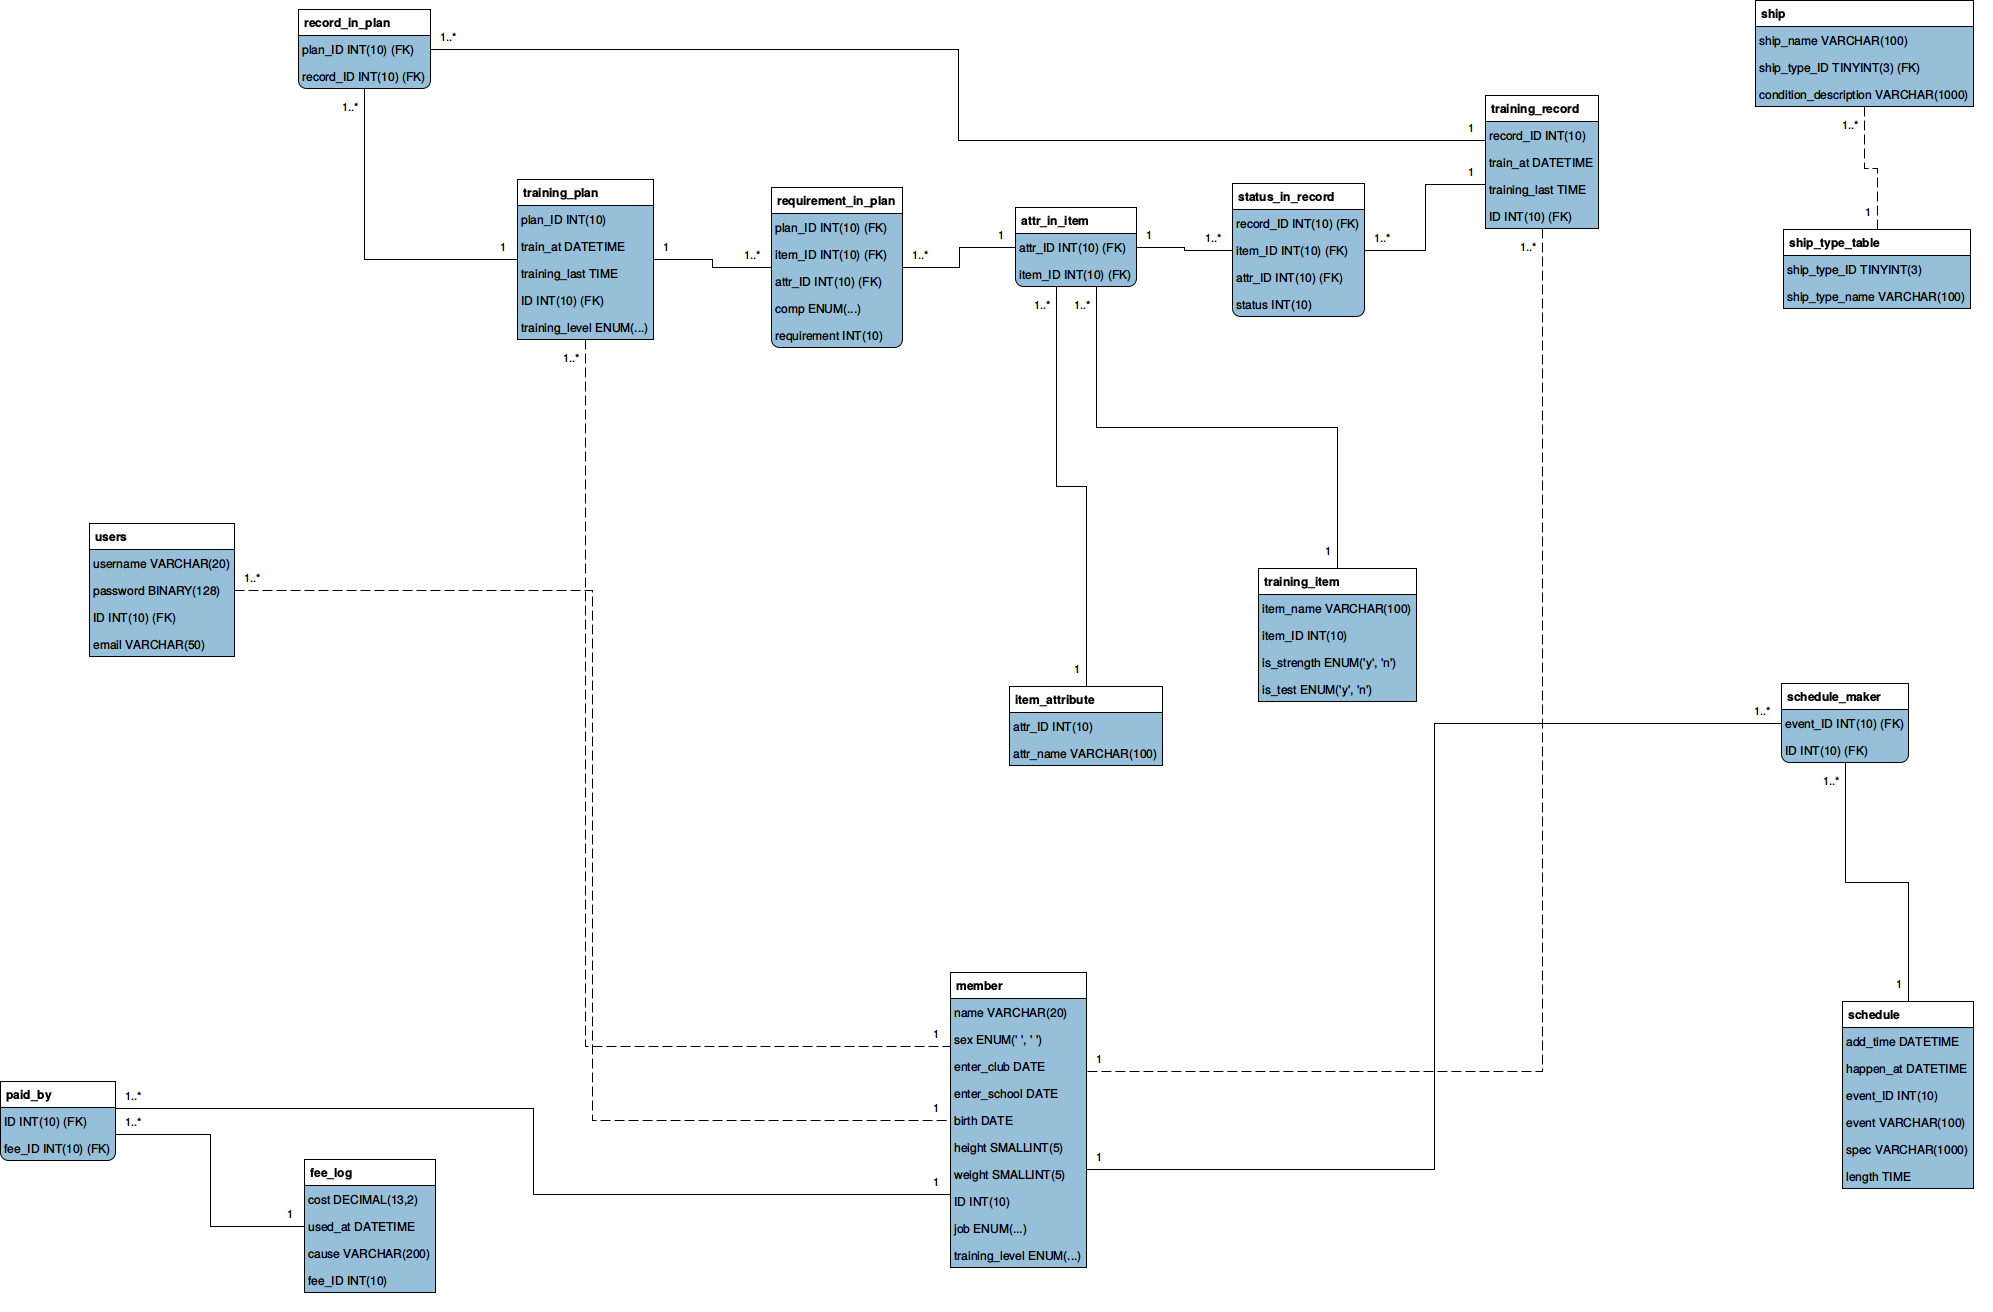
\includegraphics[width=\textwidth]{figure/relation-schema}

图中的系统层就是我们设计的网页应用。他简化了用户和数据库的交互,并提供一定的等级
分层,以及维护系统的数据完整性。

\begin{tikzpicture}
  [node distance=3cm,
  module/.style={circle, draw=blue!50, fill=blue!20,
    thick, inner sep=0pt, minimum size=2cm},
  manage/.style={rectangle, draw=blue!50, fill=blue!20,
    thick, inner sep=0pt, minimum size=1cm}]
  
  \node[module] (user)                           {用户};
  \node[module] (system) [right=of user]         {系统};
  
  \node[manage] (account) [above right=of system, yshift=1cm, xshift=2cm] {账号信息管理};
  \node[manage] (member) [below =of account, yshift=2cm] {成员信息管理};
  \node[manage] (fee) [below =of member, yshift=2cm] {开支信息管理};
  \node[manage] (ship) [below =of fee, yshift=2cm] {艇支信息管理};
  \node[manage] (training-plan) [below =of ship, yshift=2cm] {训练计划管理};
  \node[manage] (training-record) [below =of training-plan, yshift=2cm] {训练记录管理};

  %\draw [->] (system.north west) .. controls +(up:1cm) and +(up:1cm) .. (user.north east);

  \draw [->, thick] (user.north east) -- node[above] {管理} (system.west);
  \draw [->, thick] (system.west) to node[below] {信息} (user.south east);

  \draw [<->, thick] (system.north east) to (account.west);
  \draw [<->, thick] (system.north east) to (member.west);
  \draw [<->, thick] (system.east) to (fee.west);
  \draw [<->, thick] (system.east) to (ship.west);
  \draw [<->, thick] (system.south east) to (training-plan.west);
  \draw [<->, thick] (system.south east) to (training-record.west);
  
\end{tikzpicture}

    

\section{系统功能的实现}

\section{课程设计心得体会}
% 此处输入本文档的面向读者对象

% \section{参考文档}
% 此处输入在撰写本文档过程中所使用到的资源列表。

% \begin{itemize}
%     \item 《xxx系统技术协议书》,2016年12月
%     \item 《xxx系统需求说明文档》,2017年6月
%     \item 《xxx系统详细设计文档》,2017年6月
% \end{itemize}


% \section{术语与缩写解释}

% 本文档中使用到的术语缩写及其解释如下表\ref{shuyu}所示。

% \begin{table}[htb]
% \centering
% \label{shuyu}
% \begin{tabular}{p{2cm}|p{8cm}}
% \hline\hline

% \textbf{术语缩写} & \textbf{解释} \\
% \hline\hline

% 术语缩写 & 解释 \\
% \hline

% 术语缩写 & 解释 \\
% \hline

% 术语缩写 & 解释 \\
% \hline

% \hline\hline
% \end{tabular}
% \caption{本文档中出现的术语缩写及解释}
% \end{table}
